% Template for ICASSP-2020 paper; to be used with:
%          spconf.sty  - ICASSP/ICIP LaTeX style file, and
%          IEEEbib.bst - IEEE bibliography style file.
% --------------------------------------------------------------------------
\documentclass{article}
\usepackage{spconf,amsmath,graphicx}

% Example definitions.
% --------------------
\def\x{{\mathbf x}}
\def\L{{\cal L}}

% Title.
% ------
\title{Multivariate Time Series Forecasting with Dilated Kernels}
%
% Single address.
% ---------------
\name{Daniel Petterson}
\address{Victoria University of Wellington}
%

\begin{document}
%\ninept
%
\maketitle
%
\begin{abstract}
Multivariate time series forecasting plays a crucial role in various domains including traffic management, financial investment and power generation. Designing accurate forecasting algorithms can be problematic due to real-world data often involving linear dependencies as well as periodic or sequential patterns. Recent Deep Learning models such as LST-net combine the benefits of CNNs with the temporal modelling ability of RNNs to improve on more traditional autoregressive models. We aim to determine if the performance of this model can be improved through the inclusion of a dilated convolutional layer.
\end{abstract}
%
\begin{keywords}
Autoregressive models, Neural Network, Multivariate Time Series
\end{keywords}
%
\section{Introduction}

Sequential data is generated from a wide range of sources such as weather stations, traffic sensors and power plants. The values recorded over time from a singular sensor forms a series. In forecasting the goal is to take a sequence of observed values $\{X^{t-y},...X^{t-1}, X^{t}\}$ and predict future values for a pre-defined horizon, $\tau$,  $\{X^{t+1},...X^{t+\tau}\}$. As there are often interdependencies between different variables in the real world, we can model the correlations among multiple time series using multivariate time-series forecasting. The key to accurate forecasting is to account for the spatial and temporal relationships between different series at different times. Changes in one series may have a non-linear or delayed effect on the direction and magnitude of change in another and any series may be subject to seasonality such as a decreased production of energy from PV solar panels during the evening or early morning hours. This seasonality is defined as a periodic or cyclical change in values that must be taken into account in modelling. 

LSTnet\cite{lai2018modeling} has been proven to overcome many of the issues of earlier Deep Learning models used for multivariate time series problems through its novel architecture. The model combines a Convolutional Neural Network (CNN) with two separate Gated Recurrent Unit(GRU(cite author)) layers to adjust the output of a traditional autoregressive model in order to generate a prediction over the forecasting horizon. The idea behind the model structure being that convolutional layers would be to learn filters that represent repeating patterns in the series to improve the accuracy of predictions.


The remainder of this paper is outlined as follows. Section II covers the impact of LSTnet on multivariate time series forecasting. Section III describes the components of the model and our proposed modification. Section IV describes the original dataset and the one we will use for comparison. Section V discusses the experimental results. 

\section{Related Work}
RNN models have become increasingly used in multivariate time series forecasting in no small part due to the performance of models such as LSTnet as well as the increased availability of large real world datasets to train on\cite{hewamalage2021recurrent}.  Similar models that combine RNN components with more traditional forecasting techniques such as exponential smoothing\cite{smyl2020hybrid} have shown remarkable accuracy and are considered state of the art.

\section{Proposed Model}
\begin{figure}[htb]
	
	\begin{minipage}[b]{1.0\linewidth}
		\centering
		\centerline{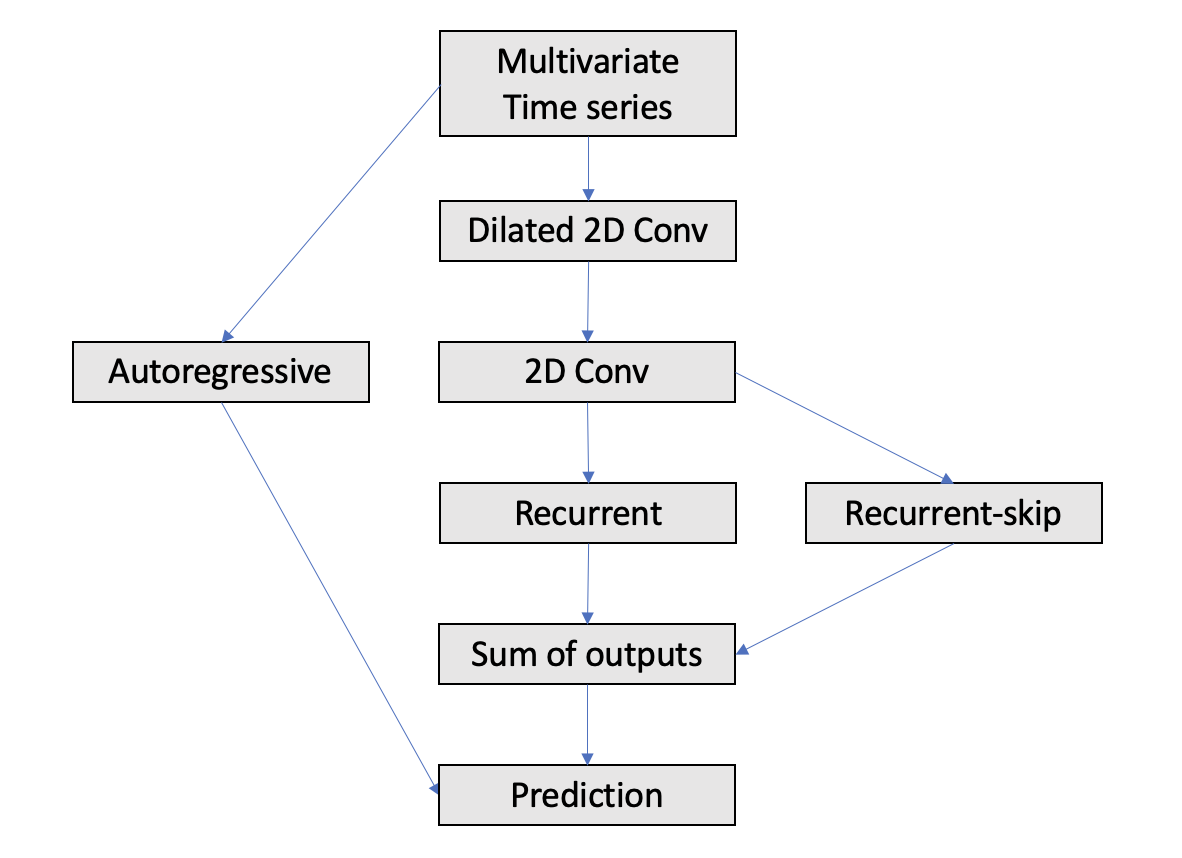
\includegraphics[width=8.5cm]{model_struct}}
		%  \vspace{2.0cm}
		\centerline{(a) Proposed Model Structure}\medskip
	\end{minipage}
\end{figure}
We propose the addition of a 2 dimensional dilated convolutional layer to the architecture of LSTnet in an attempt to improve the accuracy of predictions. As per our proposed structure, the dilated convolutional layer will precede the convolutional layer of the original model. For the purpose of this experiment we will use the dilation rate of two. The Rectified Linear Unit will be used as the activation function for every non-autoregressive component.



\subsection{Convolution Component}
In the original model there is a single convolutional layer that takes the time series data as input and applies a kernel of dimensions, ($H,  W$) where $W$ is the kernel size and $H$ is the number of series, across the input matrix. Each kernel is composed of a number of filters and we generate the output by sliding a filter, or weight matrix, over the input and at each point computing the dot product between the two. This component allows the model to learn filters that are able to recognize specific patterns in the input data.

The model we propose (LST-dil) has a additional dilated convolutional layer that feeds into this aforementioned layer. Dilated convolution works similarly to traditional convolution but the kernel is expanded by the factor of the dilation by skipping input variables so that in the case of multivariate time series, a kernel of dimensions ($n$,$m$)  and a dilation rate of $p$ would convolve values on every $p^{th}$ step over a range of ($p*n$, $p*m$) This allows for a larger receptive field including a greater range of time points. Dilated convolution been associated with impressive results from models such as WaveNet and we aim to investigate whether using a dilation rate of greater than one will allow better recognition of patterns in the data.

\subsection{Recurrent/Skip Recurrent Components}
The Recurrent and Skip Recurrent layers both take input from the final convolution layer. The Recurrent layer is constructed with Gated Recurrent Units (GRU) \cite{chung2014empirical} which offers a helps to mitigate the issue of exploding or vanishing gradients caused by long products of matrices. GRUs are not perfect though and have issues capturing very long-term correlations that can be present in time series data. To remedy this, the Skip-RNN layer, skipGRU, only takes input from every $nth$ step where $n$ is defined as the length of a period or season. Looking at traffic data, we would set $n$ to compare the value of a series at time $t$ to the values of $t$ in previous weeks. This allows the capture of seasonality from both the changes throughout a single day but also the changes that occur on the weekends. The outputs of the GRU and SkipGRU layers are joined and fed through a fully connected layer of size one before being summed with the linear component to be discussed in Section 3.3.


\subsection{Autoregressive Component}
The traditional Autoregressive (AR) model is employed as the linear component of this model which is required as the other components are insensitive to nonperiodical changes in the scale of the input data and thus liable to underperform if that changes significantly. The AR component can be thus thought of as the baseline over which the output of the GRU layers are added to account for reoccurring patterns or seasonality. The output of the Autoregressive component is as follows,
\begin{align}
x^i = \sum_{t'=T-window}^{T-1} W_{t'}^{i} X_{t'}^{i} +B^{i} 
\end{align}
\begin{align}
out = concat(x^1,x^2,x^3...x^i) 
\end{align}
where $i$ denotes the number of series, $X_{t'}^{i}$ denotes the $i^{th}$ input at time $t'$, $W_{t'}^{i}$ denotes the corresponding weight matrix, $b^i$ is the bias and $window$ is the time window of the AR model.
 
\section{Evaluation}
Our model was implemented on the Tensorflow framework as was the baseline configuration of LSTnet for a fair comparison. In this we introduce the dataset used in this experiment and the evaluation methods and parameters of the models. The training parameters will be the same as the original implementation(cite research paper) and the models shall be trained for 100 epochs on the first 60\% of the time series while the remaining 40\% of the series shall be split evenly between validation and testing sets respectively.

\subsection{Metrics}
We make use of two metrics to compare model performance, the Root Relative Squared Error (RSE):
\begin{align}
RSE = \frac{\sqrt{\sum_{(i,t\in\Omega Test)}(Y_{it}-\hat{Y_{it})}^2}}{\sqrt{\sum_{(i,t\in\Omega Test Y_{it}-mean(Y))^2}}}
\end{align}

and Pearson's r (Corr):
\begin{align}
r = \frac{n(\sum xy) - (\sum x)(\sum y)}{\sqrt{[n\sum x^2-(\sum x)^2][n \sum y^2-(\sum y)^2]}}
\end{align}
Time series forecasting can be viewed as standard regression problems with time-varying parameters making the correlation a telling metric of a model's performance\cite{kim2003financial, cao2003support}. A higher Pearson's R indicates better performance and the opposite is true for RSE. The RSE is a scaled version of the more popular Root Mean Square Error(RMSE) which provides more readable results. 

\subsection{Data}
The data consists of hourly measurements of road occupancy on San Francisco Bay area motorways from 25 sensors. It was collected over 24 months (2015-2016) by the California Department of Transportation and the original dataset with values from all 862 sensors is publicly available.

\subsection{Experimental Results}


\begin{table}[!h]
	\renewcommand{\arraystretch}{1.3}
	
	\label{netstructtab}
	\centering
	\begin{tabular}{ll|ll}
		\hline
		&         & \multicolumn{2}{l}{Horizon} \\ \hline
		Model   & Metrics & 12           & 24           \\ \hline
		LST-net & RSE     &    1.8916         &     1.7860         \\ 
		& Corr    &      0.8390       &        0.8720     \\ \hline
		LST-dil & RSE     &     2.3198          &    2.3503          \\ 
		& Corr    &      0.7551         &        0.7471      \\ \hline
	\end{tabular}
\caption{Summary of Results}
\end{table}

Our proposed model, LST-dil performed poorly on the dataset compared to the baseline, LSTnet at a horizon of both 12 and 24 hours. 

\section{Conclusion}
The model we proposed performed worse across both metrics and horizons trialed. The additional dilated convolutional layer had a negative impact on the ability of the model to accurately forecast future values. We may have seen better results by modifying the parameters of the layer or increasing the number of dilated layers.



\vfill\pagebreak


\bibliographystyle{IEEEbib}
\bibliography{strings,refs}

\vfill\pagebreak

\section{Appendix}
The accompanying code can be found in a Colab Notebook at the following link:
https://colab.research.google.com/drive/1VRMnv1Sq15gXXmyBECwCQJDe56u21k5g?usp=sharing



\end{document}
